\documentclass[scheme=plain,12pt]{ctexart}

\usepackage{graphicx}
\usepackage[hmargin=1.1in,vmargin=1in]{geometry}
\usepackage{indentfirst}

\fontsize{14pt}{1.0}

\newlength{\blanklength}
\setlength{\blanklength}{40ex}

\providecommand{\thetitle}{Overview of Advanced Data Structures}
\providecommand{\theauthor}{Sparky\_14145}
\providecommand{\thestudentID}{71XXXXXX}
\providecommand{\theemail}{Sparky\_14145@outlook.com}
\providecommand{\theinstitution}{College of Software Engineering}

% \input{personal_info/info.tex}

\providecommand{\blankToFill}[1]{
    \parbox[t][3ex]{\blanklength}{
        \makebox[\blanklength]{#1}\\[0pt]
        \rule[2ex]{\blanklength}{0.1ex}
    }
}

\providecommand{\makecover}{\begin{titlepage}
    \noindent
    {Course Report} \\[2pt]
    {\large \bfseries Southeast University}

    \vspace*{20pt}
    \begin{center}
    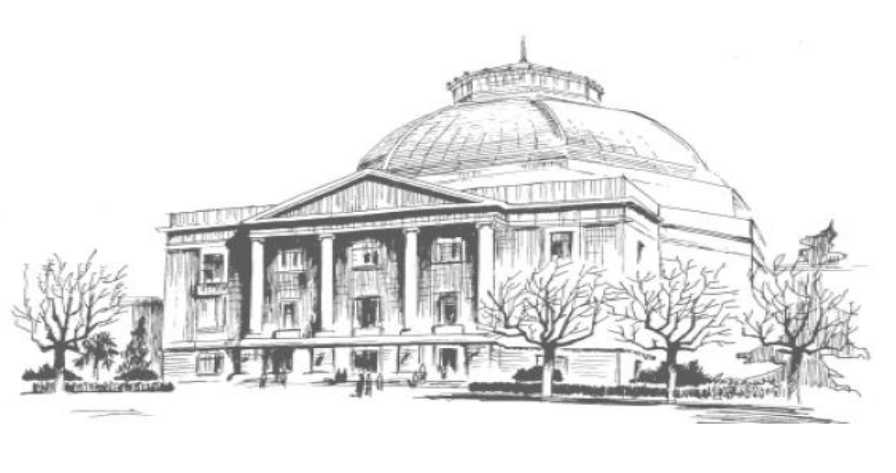
\includegraphics[width=0.8\textwidth]{pics/cover.png}
        \textsc{\Huge Advanced Data Structures}

        \vspace*{10pt}
        \begin{tabular}[c]{rc}
            Title       & \blankToFill{\thetitle} \\
            Date        & \blankToFill{\today} \\
            Author      & \blankToFill{\theauthor\footnotemark} \\
            Student ID  & \blankToFill{\thestudentID} \\
            Institution & \blankToFill{\theinstitution}
        \end{tabular}
        \rmfamily
    \end{center}

    \vspace*{0pt}
    \begin{abstract}
        Advanced data structures are the data structures that have advanced features,
        like staying effective without using extra storage space (\emph{Splay trees}),
        holding persistent data while having short access and modify time (\emph{Persistent
        Segment trees}) or easy to implement but fast to use in most situations (\emph{Skip
        lists}). Advanced data structures are invented to solve different problems that
        the data structures before cannot solve, so there is no ``universal'' ways to
        make a data structure ``advanced''. but there are still some common thoughts in parts
        of these structures, like their ways to hold persistent data and their ways to reduce
        complexity of operations. Like all other things, the advanced data structures are
        under continous development. The trends of advanced data structures are: they are
        going to be more and more complex (both in relationships between data and in algorithms
        to access and maintain the structures), they are more and more running on distributed
        systems and decentralized environments.
    \end{abstract}
    \footnotetext{\theemail}
\end{titlepage}}

\begin{document}
    \makecover

    \section{Introduction}

    \noindent
    Wikipedia says:

    \begin{quotation}
        A data structure is a collection of data values, the relationships among them, and 
        the functions or operations that can be applied to the data, i.e., it is an algebraic
        structure about data. 
    \end{quotation}

    Data structures stores data, in an organized way, so that programs can use the data well.

    \subsection{Why advanced data structures}

    Basic data structures, like basic array, linked list, stack, queue and so on, offer basic
    ways to organize data. They are really generic, and used quite widely. However, as our
    experience told to us, the more generic sth. is, the less effective it is, and the basic
    data structures cannot always meet our requirements, especially when the quantity of data
    is huge, or the space or time of applying operations is limited. We need some more effective
    ways to organize our data!

    \subsection{From basic data structures to advanced data structures}

    As is mentioned above, basic data structures has lots of constraints. With the world changes
    fast, users of softwares have more and more requirements, including but not limited to
    efficiency, reliability, trustlessness and decentralization. 

    There are some extreme situations that basic data structures cannot work well:

    \begin{enumerate}
        \item Size of data is huge. The quantity of data is so big that the data structure itself
              cannot be stored in the memory entirely, like snapshots of most websites on the
              Internet used by search engines;
        \item Response time needs to be very short. The response time of the program needs to be
              so short that $O(n)$ access time in a single operation is unbearable, otherwise the
              users may feel noticeable lag and feel dissatisfied;
        \item Operations can be undone fast. Sometimes users may wish to undo their last operations,
              like rolling back the database, and sometimes the operations to undo may be massive
              like rolling back to a specific version in Version Controlling Systems.
    \end{enumerate}
    
    The requirements drives CS scientists to find new ways to compute or process data better (by
    improving or inventing algorithms) and to organize the data better (by advancing data
    structures).

    \subsection{What are advanced data structures}

    Advanced data structures are also data structures. They are also consists of three parts:
    the data, the relationships (between the data), and the algorithms (to get and maintain the
    data). However, advanced data structures are \emph{advanced} by scientists, making them
    suitable for hard tasks that challenges the data structures' functions and efficiency severely.

    The word \emph{advanced} in the \emph{advanced data structures} is not only an adjective,
    but also a verb. It means that the data structures are \emph{advanced}, or \emph{improved},
    in some way, so that it can be capable for some hard tasks.

    In some advance data structures, the only things changed are algorithms used to maintain.
    The data and relationship are not changed, like \emph{Splay trees} does not change fields
    stored in the nodes. The other ones, like \emph{Red-Black trees}, attaches additional data
    and relationships to the data structures, to help improving the algorithms to maintain.

    \section{Common thoughts in advance data structures}

    There are lots of common thoughts in advanced data structures, here we list some examples of them.

    \subsection{Ways to hold persistence data}

    Persistence is a thought that tries to make the data structures can be ``rolled back''.

    To achieve this, there are also lots of solutions:

    \begin{itemize}
        \item Copy-on-write. Coping the whole data structure after each modification. This is
              easy to implement, and have the shortest access time, but requires lots of time
              (on coping the structure) and space (to store the duplicates) to apply the
              modifications;
        \item Fat node. Each node maintains a list that stores its changes. When a modification
              is done on a node, the old data is not modified. Instead, the new data and its
              version stamp is appended to the tail of the list. This is also easy to implement,
              and requires minimal space and time to store when each modification only involves
              a small amount of nodes (since each modification is done at a $O(k)$ cost, $k$ is
              the count of involved nodes). But when $k$ becomes huge, the cost can be also
              noticeable;
        \item Path copying. After a modification, all nodes on the path to the modified nodes
              are copied, while modifying all nodes point to the old points to the new ones.
              This algorithm is more complex than the two above, but balance the access time
              and the modify time best;
        \item Combination. By combining the algorithms above, we can take advantages of each one.
              For example, the most common implementation of \emph{persistence segment tree},
              maintains the root as a fat node, while applying path copying to the whole tree,
              to keep the data structure effective.
    \end{itemize}

    \subsection{Ways to reduce complexity of operations}

    \subsubsection{Amortizing the long time of several operations to other ones}

    If the access operations of a situation does not need to be always as fast as possible,
    amortizing the time of each operations, to strike a good balance between space and total
    time could be a good idea. Here are two examples of amortization:

    \begin{itemize}
        \item Vectors. Vector is a type of linear list, whose length is not fixed. When appending
              elements to the end of a vector, if there is no enough pre-allocated space to
              store, the vector automatically requires space $k (k > 1)$ times more than before.
              Though sometimes an insertion takes $O(n)$ time (where $n$ is the pre-allocated
              space of the vector), the amortized time of each insertion is still $O(1)$, so
              vector is still a effective data structure;
        \item Splay trees. Splay trees try to make a simple reconstruction, to optimize the
              future operations. It rotates the accessed node to the root after each operation.
              Each access operation or modify operation may take $O(n)$ time to perform, but they
              are $O(\log n)$ in amortization, enabling Splay trees stay effective while do not
              need extra space to store information to keep balanced, or \emph{almost} balanced.
    \end{itemize}

    \subsubsection{Randomizing the relationship between the data}

    Assign random priority or weight to items in the data structure, so that the data structure
    can have a good performance in expectation. Though situations that the structures can lose
    their efficiency exist, but the greater size of data is, the smaller the chance is. So in
    most situations, these structures are still effective enough. Here are two examples:

    \begin{itemize}
        \item Treap. Treap is a self-balanced binary search tree. In addition to the original
              data, treap assigns an extra field, priority, to each node. Treap tries to organize
              its nodes like a heap, when considering the priorities. So if the priorities are
              assigned randomly, the tree is expected to be balanced, granting the data structure
              efficiency;
        \item Skip list. Skip list is a multi-level linked list. Each item in the list have a
              chance to be ``upgraded'' to higher level, so that when accessing, we can start
              from the higher level to ``skip'' some items, fastening the access speed. The
              $n$-th level is expected to have $\frac{n}{q^{n-1}}$ items, so that each access
              operations are expected to be $O(\log n)$.
    \end{itemize}

    \section{Trends of advanced data structures}

    With the world developping faster and faster, the demands and the requirements to the
    softwares are changing, driving the advanced data structures evolving. Here are several
    trends the advanced data structures have in the near future:

    \subsection{Becoming complicated}

    On the one hand, the size of data, the size of information on the Internet, is experiencing
    a exponential explosion. The huge size of data requires better performance on data processing
    and accessing, leaving old algorithms and data structures out of date faster and faster; On
    the other hand, the relationship between data is also being more and more complicated: We
    may need to research lots of different relationships on the same data set on the same time.
    So old data structures that only maintain 1 dimension of relationships are discarded.

    For example, the database softwares need to be able to search or sort several records by
    different keys. In this situation, traditional binary search trees cannot satisfy the
    requirements, and advanced data structures, even several combination of advance ones, are
    used instead.

    \subsection{Running on distributed systems}

    Sometimes the size of data is just too big to store in the memory, and the data structure
    have to store parts of itself in the disks, sometimes even remote disks on the network.
    In such situations, \emph{B-trees} and \emph{R-trees} were invented, they can stores parts
    of themselves not in the memory, while offering good performance on searching and indexing.

    And sometimes a single computer can only offer a limited computing capability due to
    limited hardware technology, so a group of computer, or say a \emph{computing cluster} is
    needed to fit the computing requirements. \emph{MapReduce Frameworks} and other high
    performance computing frameworks are solutions to this. They try to give proper tasks
    to each computer in the cluster, so that the advantages of parallel computing could be
    taken.

    \subsection{Running on decentralized environments}

    Traditional applications require central servers to prove that the data is valid. But in
    some cases, for example Bitcoins and Certification Authority of web browsers, trusting a
    third-party server unconditionally may not be a good idea. So decentralized data structures
    were invented. They try to attach additional information to the known data structures,
    so that illegal modification can be recognized and prevented.
\end{document}